% This is the file main.tex
\usepackage{group4}

\begin{document}
	
	\mode<article>{
		\newgeometry{margin=2in}
				\maketitle
				\restoregeometry
				\thispagestyle{empty}
				\newpage
				
				\textit{The following is just a collection of the discussions in preparation for turning what we have done into a write-up. This is not an actual write-up.}
		}
	
\begin{frame}
  \titlepage
\end{frame}

\titlepage

\mode<presentation>{
\section*{Outline}
\begin{frame}{Outline}
  \tableofcontents
\end{frame}
}

\mode<article>{
	\section{Achieving Stationarity}
	
	\subsection{Testing for Stationarity}\begin{itemize}
		\item I performed the ADF (augmented Dickey-Fuller) test for stationarity. We haven't talked about it in class yet, but it seems to be used pretty commonly. The high p-value suggests that we do not have a stationary model with just the raw unemployment data. This is confirmed with the non-constant variance and time-dependent mean that we observed in our exploratory analysis.\\


\begin{center}
	\textbf{Augmented Dickey-Fuller Test}\\
\end{center}
\begin{multicols}{2}
	
data:  unem\\
Dickey-Fuller = -1.4266, Lag order = 6, \\
p-value = 0.8176\\
alternative hypothesis: stationary\\


data:  unem.sa\\
Dickey-Fuller = -2.1377, Lag order = 6, \\
p-value = 0.518\\
alternative hypothesis: stationary\\
\end{multicols}

	
	\subsection{Initial Plots}
	
			
\begin{figure}[H]
\centering
\caption{Plot of the original data}
\label{fig:unemployment}
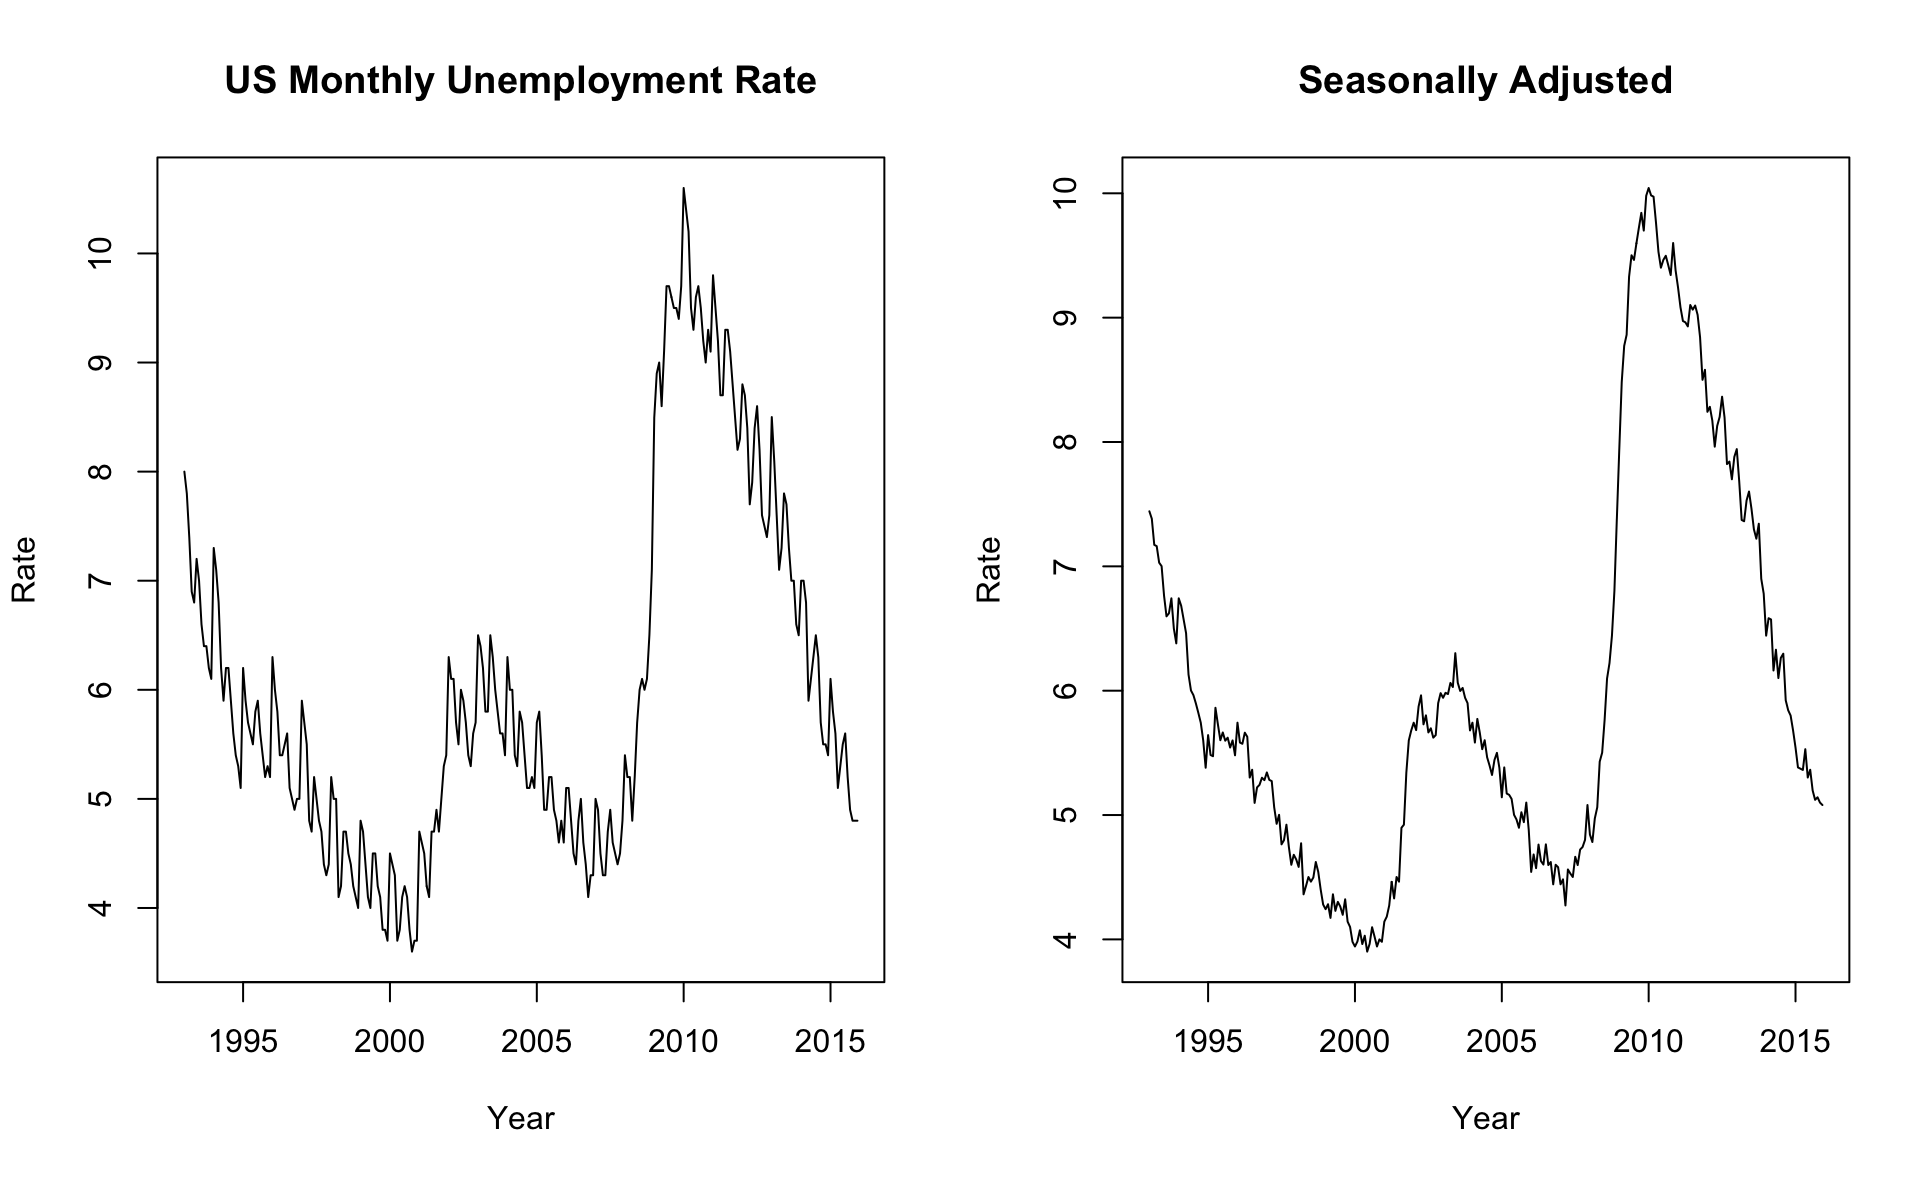
\includegraphics[width=\linewidth]{images/Unemployment}
\end{figure}

			
			\begin{multicols}{2}
						I then plotted the first difference, and it appears relatively stationary.\\
						
							This is confirmed by the ADF test on the first differenced data, which has a very small p-value:\\
						
						Augmented Dickey-Fuller Test\\
						Dickey-Fuller = -4.3501, Lag order = 6, p-value = 0.01\\
						alternative hypothesis: stationary
						
						\begin{figure}[H]
							\centering
							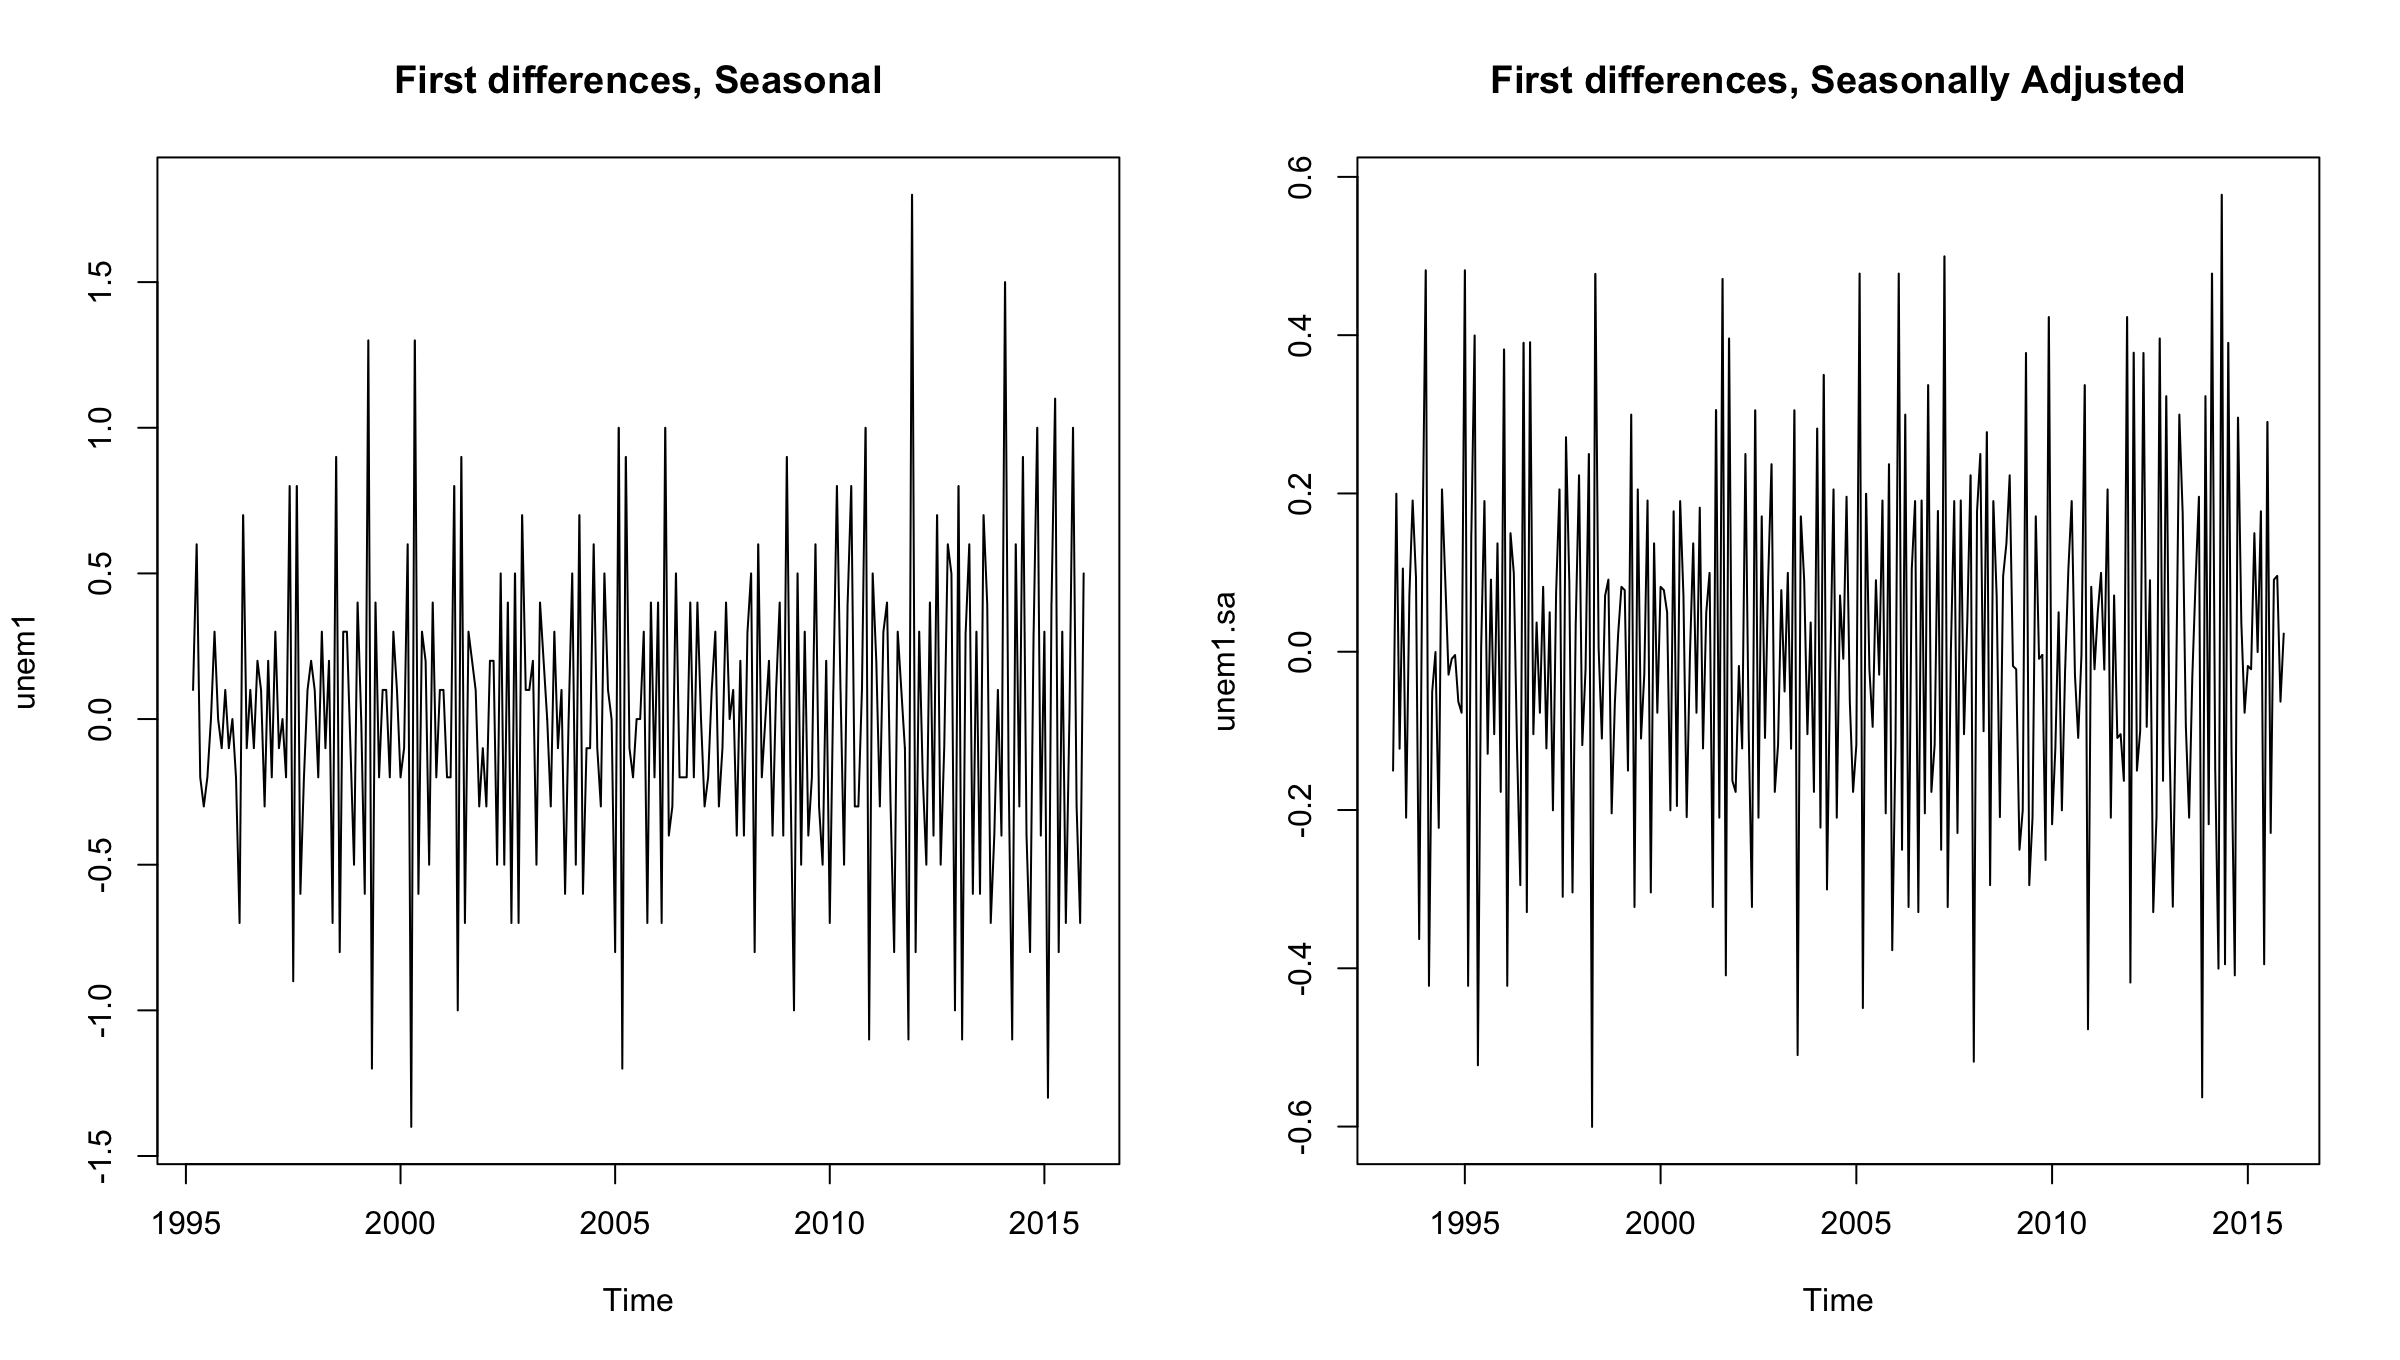
\includegraphics[width=.6\linewidth]{images/firstdiff}
							\caption{Plot of first Difference}
							\label{fig:firstdiff}
						\end{figure}
			\end{multicols}
			


		\end{itemize}	}
	


\mode<presentation>{\section{Initial Plots}}

%-----------------------------------------------------------------------------------------
  \subsection{Differencing}
  
      I took the second difference (d = 2), as Joseph suggested, then the first seasonal difference (D = 1) with s = 12 (this is common for monthly economic data), as the book did. \\
      
      Below, Figure \ref{fig:secdiff},  is the plot of the transformed graphed. It looks pretty stationary (not perfect, but adequate), and we can confirm this with the ADF test (it's cited in other time series texts, but I haven't seen it in ours yet).\\
      
      \textit{I like the idea of using the ADF. We can include it as part of our literature review.}
      
      
      \begin{figure}[H]
      	\centering
      	\caption{Second differences with and without seasonal adjustments}
      	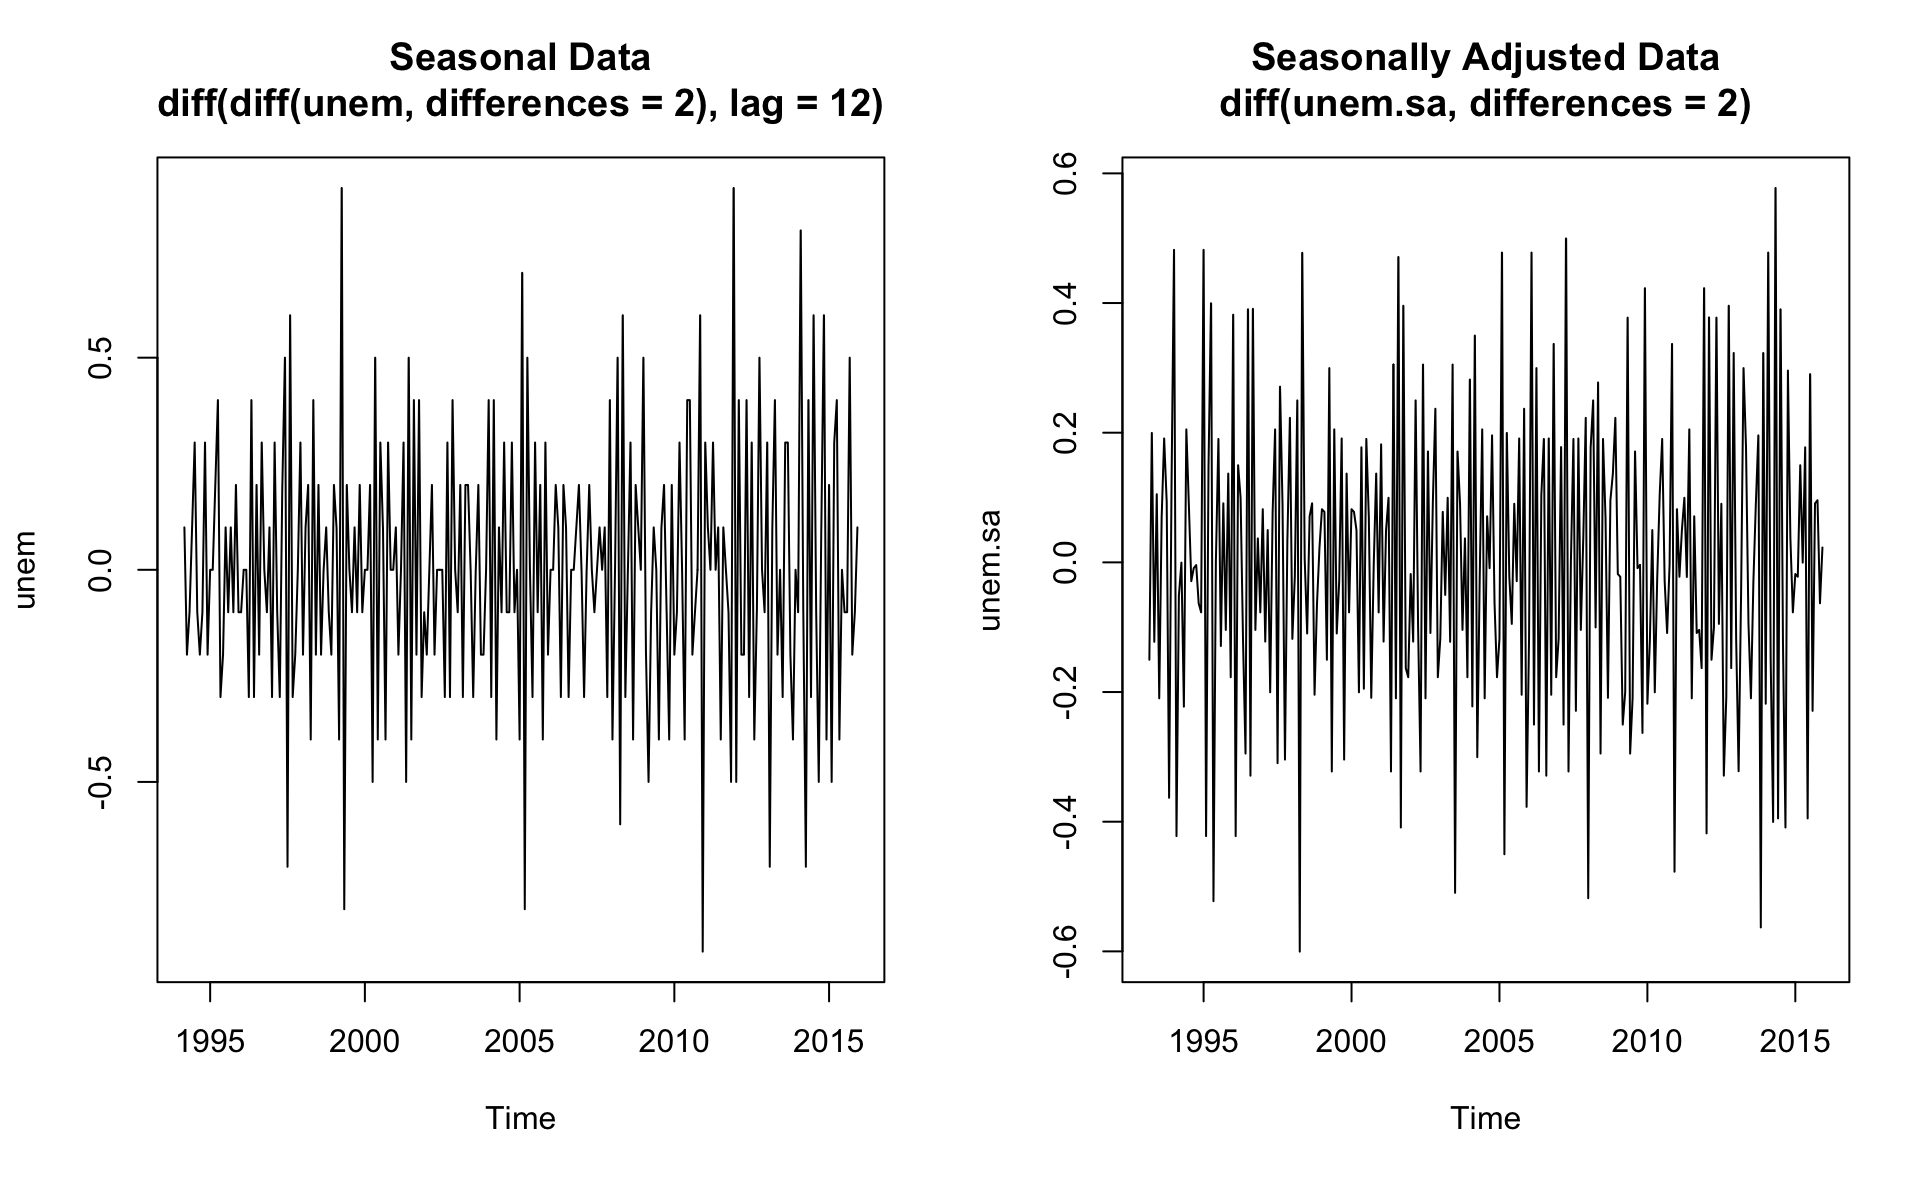
\includegraphics[width=.7\linewidth]{images/stationarity}
      	\label{fig:secdiff}
      \end{figure}
      

    

  
  \mode<presentation>{
  	\begin{frame}{Second differences with and without seasonal adjustments}
  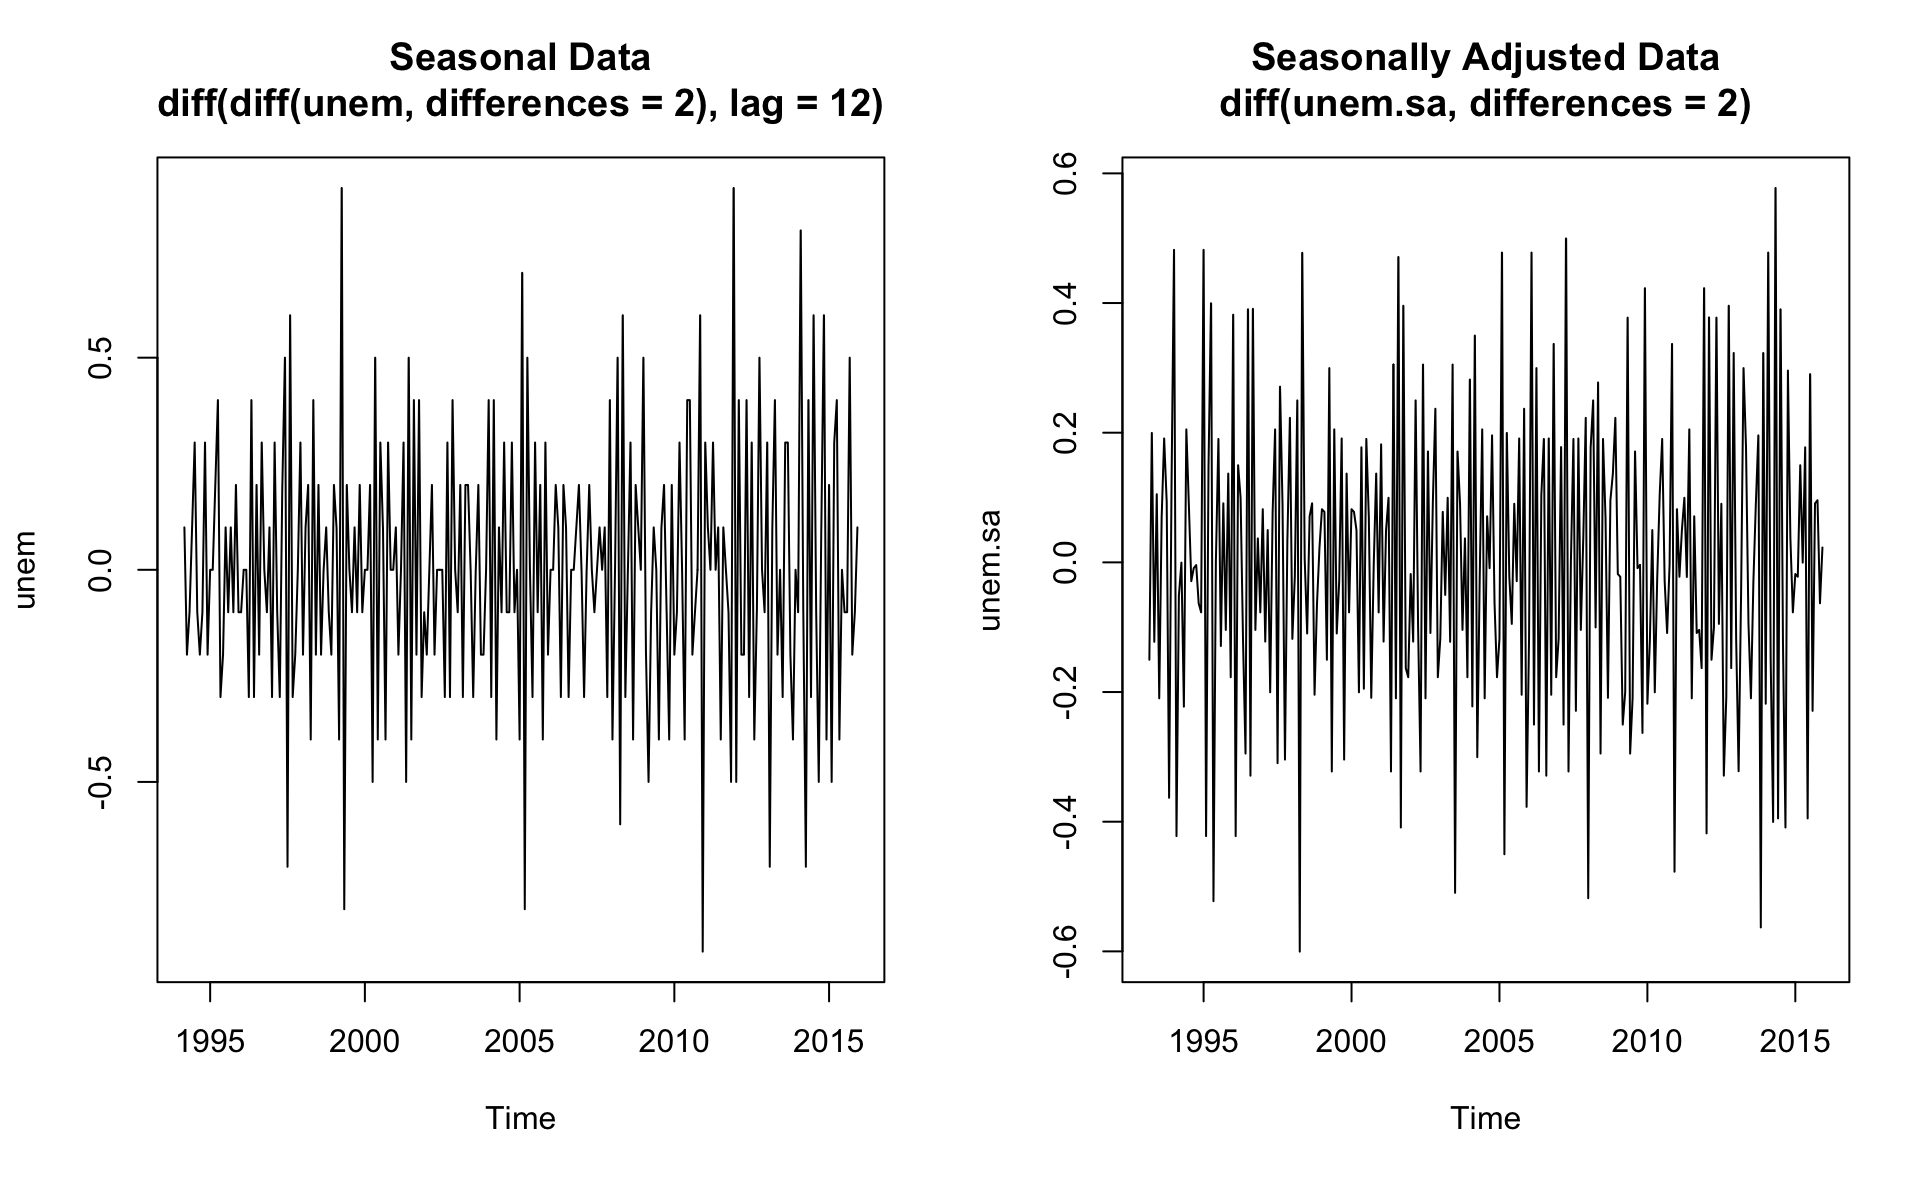
\includegraphics[width=.9\linewidth]{images/stationarity}
  \end{frame}
  }
  

%-----------------------------------------------------------------------------------------
  
  \subsection{ACF \& PACF}
  
  After that, the book suggests that you examine the ACF and PACF plots.\\
  
  First, the book says to look at the seasonal changes in ACF and PACF (h = 12, 24, 36, ...). These seem to indicate that the ACF trails off, and the PACF cuts off after one year (h = 12). This suggests that we let P = 1 and Q = 0.\\
  
  Next, the book says to look at the ACF and PACF within only the first season (h = 1, 2, ..., 12). The PACF declines slowly, but the ACF cuts off after 1, suggesting we let p = 0, and q = 1.\\
  
   \mode<presentation>{
   	 \begin{frame}{ACF \& PACF Plots}
  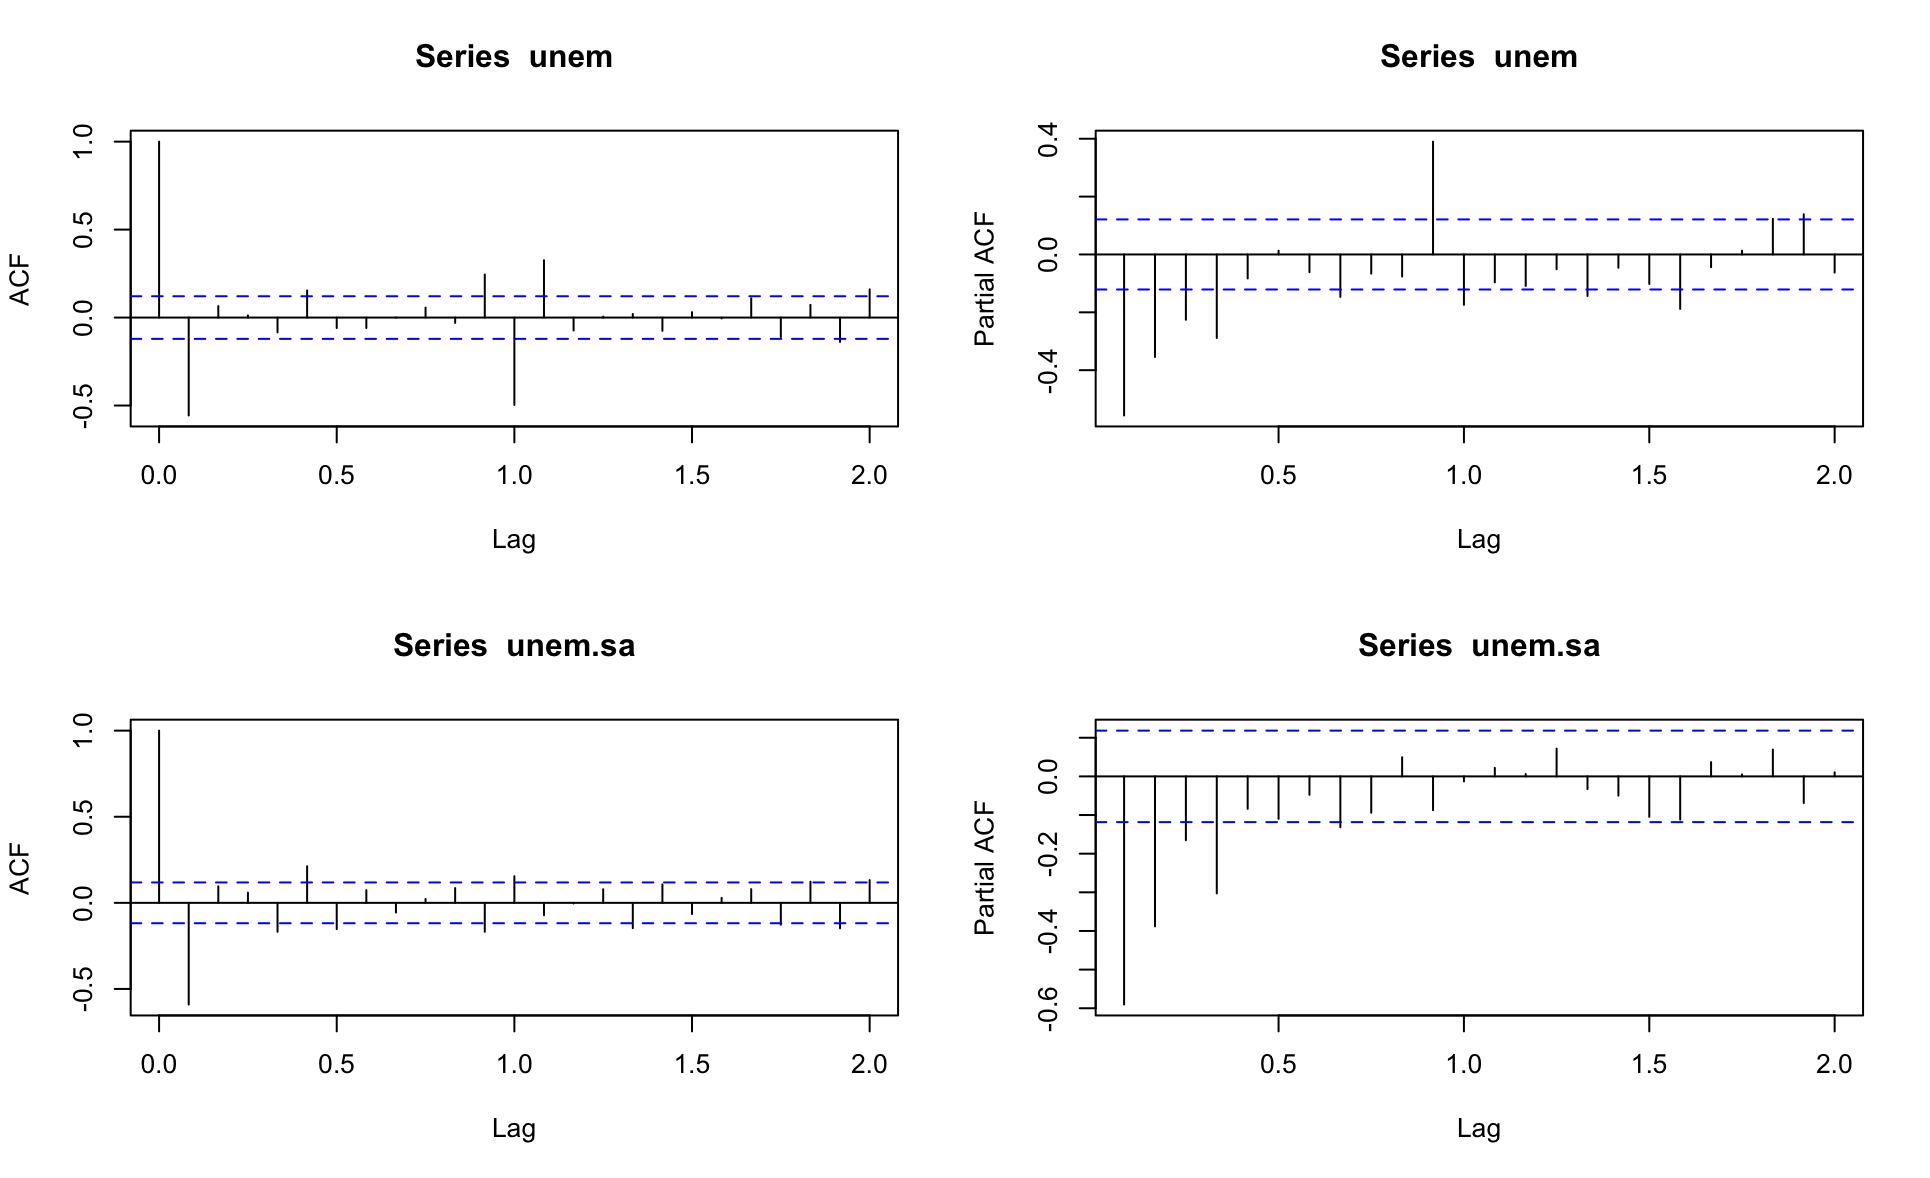
\includegraphics[width=.9\linewidth]{images/acfpacf}
  \end{frame}
}

      \begin{figure}[H]
      	\centering
      	\caption{ACF \& PACF Plots}
      	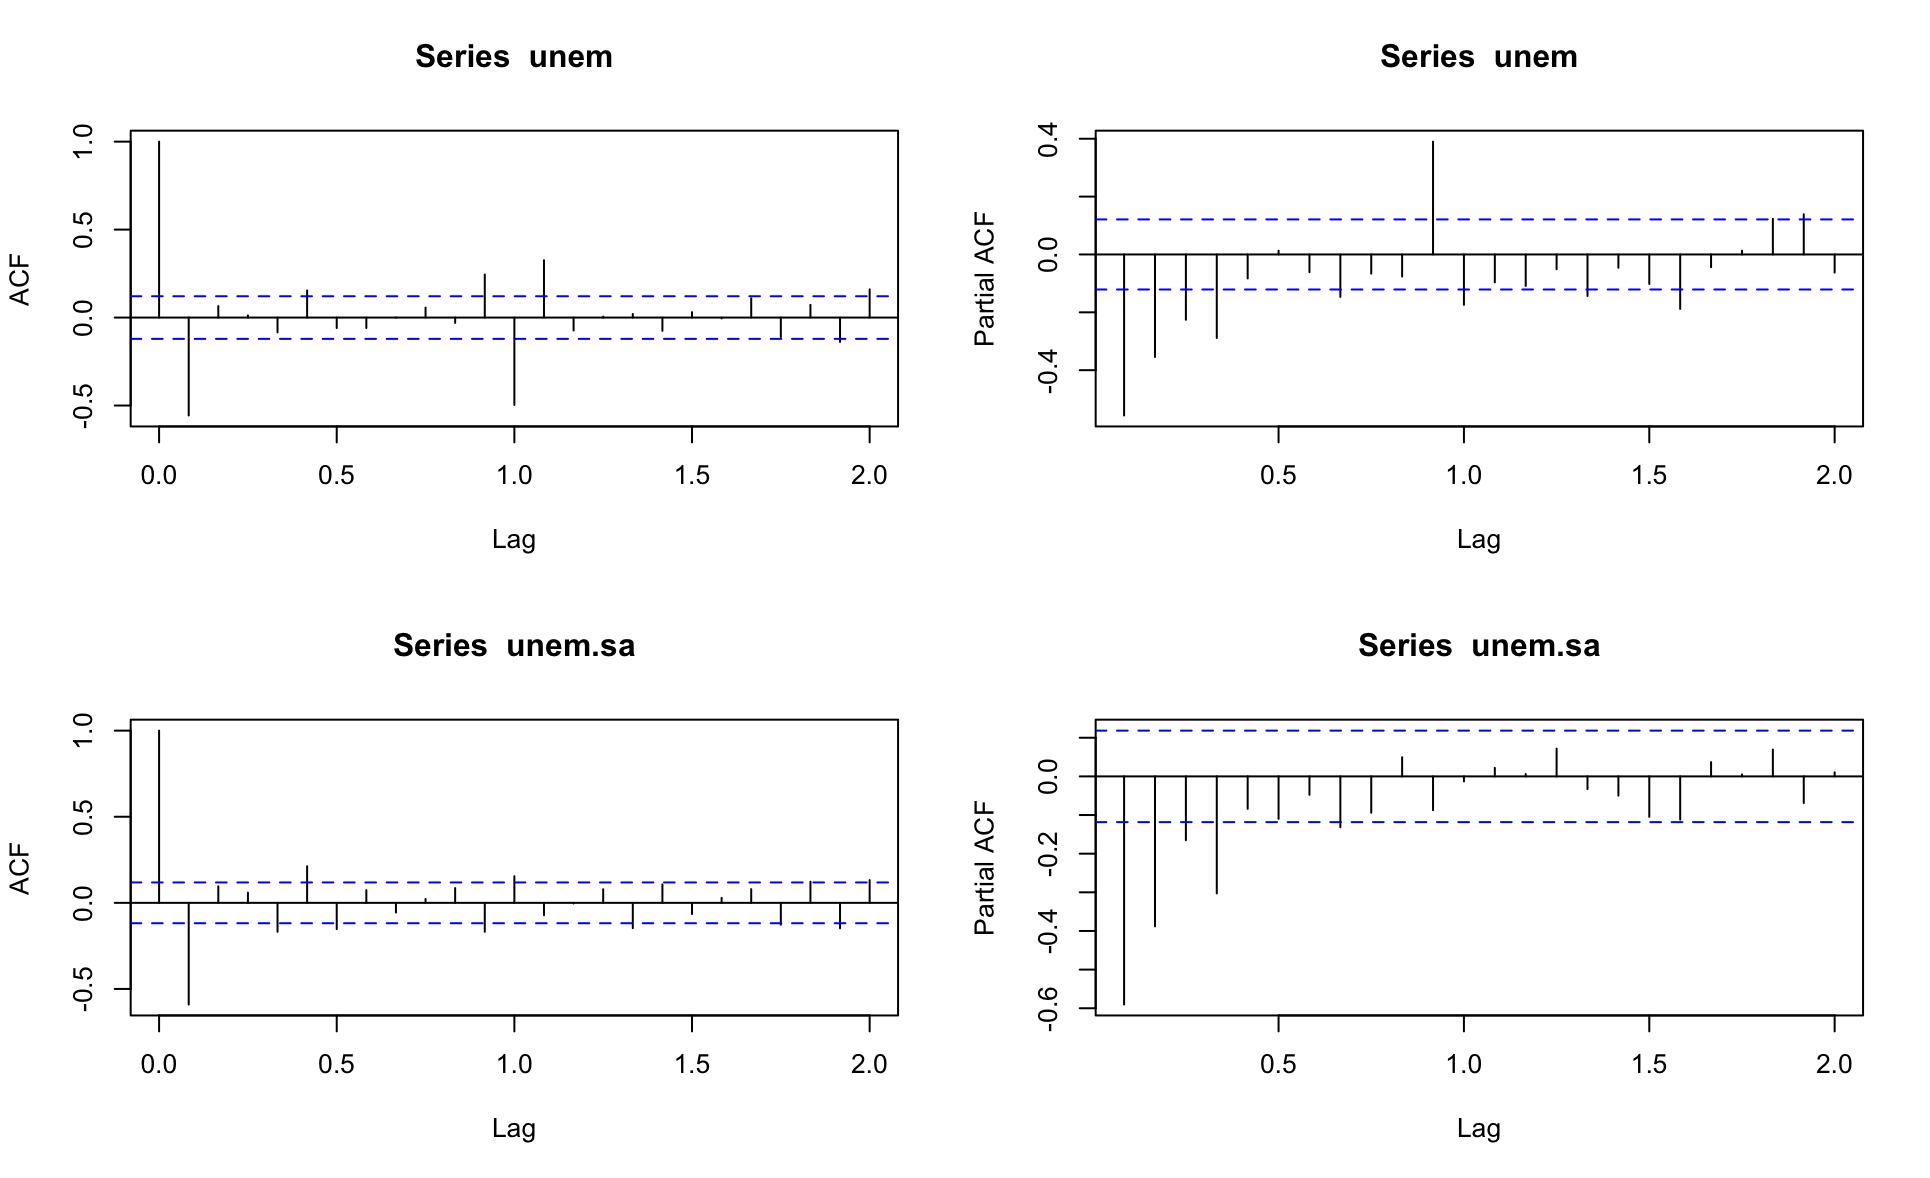
\includegraphics[width=\linewidth]{images/acfpacf}
      	\label{fig:secdiff}
      \end{figure}
%----------------------------------------------------------------------------------------- 

    \section{Model Comparisons}
    
%-----------------------------------------------------------------------------------------    
    \subsection{Overview}
  \begin{frame}{Models Considered}
    % latex table generated in R 3.2.4 by xtable 1.8-2 package
% Thu Jul  7 16:13:24 2016
\begin{table}[H]
\centering
\caption{Model Summaries}
\begin{tabular}{llccccc}
  \hline
 \textbf{\#}& \textbf{Data}  & \textbf{Order} & \textbf{Seasonal} & \textbf{XRegs} & \textbf{AIC} & \textbf{BIC} \\
 &&&\textbf{Order}&&&\\ 
  \hline
1 & Unem  & 0,2,1 & 1,1,0 & N & -2.27 & -3.23 \\ 
  2 & Unem  & 0,2,1 & 3,1,0 & N & -2.44 & -3.37 \\ 
  3 & Unem  & 4,2,1 & 3,1,0 & N & -2.44 & -3.32 \\ 
  4 & Unem.sa & 0,2,1 & 1,0,0 & N & -2.61 & -3.58 \\ 
  5 & Unem.sa  & 1,2,1 &  & N & -2.63 & -3.60 \\ 
  6 & Unem.sa & 0,2,1 & 1,0,0 & Y & -2.58 & -3.49 \\ 
  7 & Unem.sa  & 1,2,1 &  & Y & -2.60 & -3.49 \\ 
   \hline
\end{tabular}
\label{tab:models}
\end{table}
  \end{frame}
%-----------------------------------------------------------------------------------------

 \subsection{Seasonal Models}
 %-----------------------------------------------------------------------------------------
  \begin{frame}{Model 1: SARIMA\((0,2,1) \times (1,1,0)_{12}\)}
  		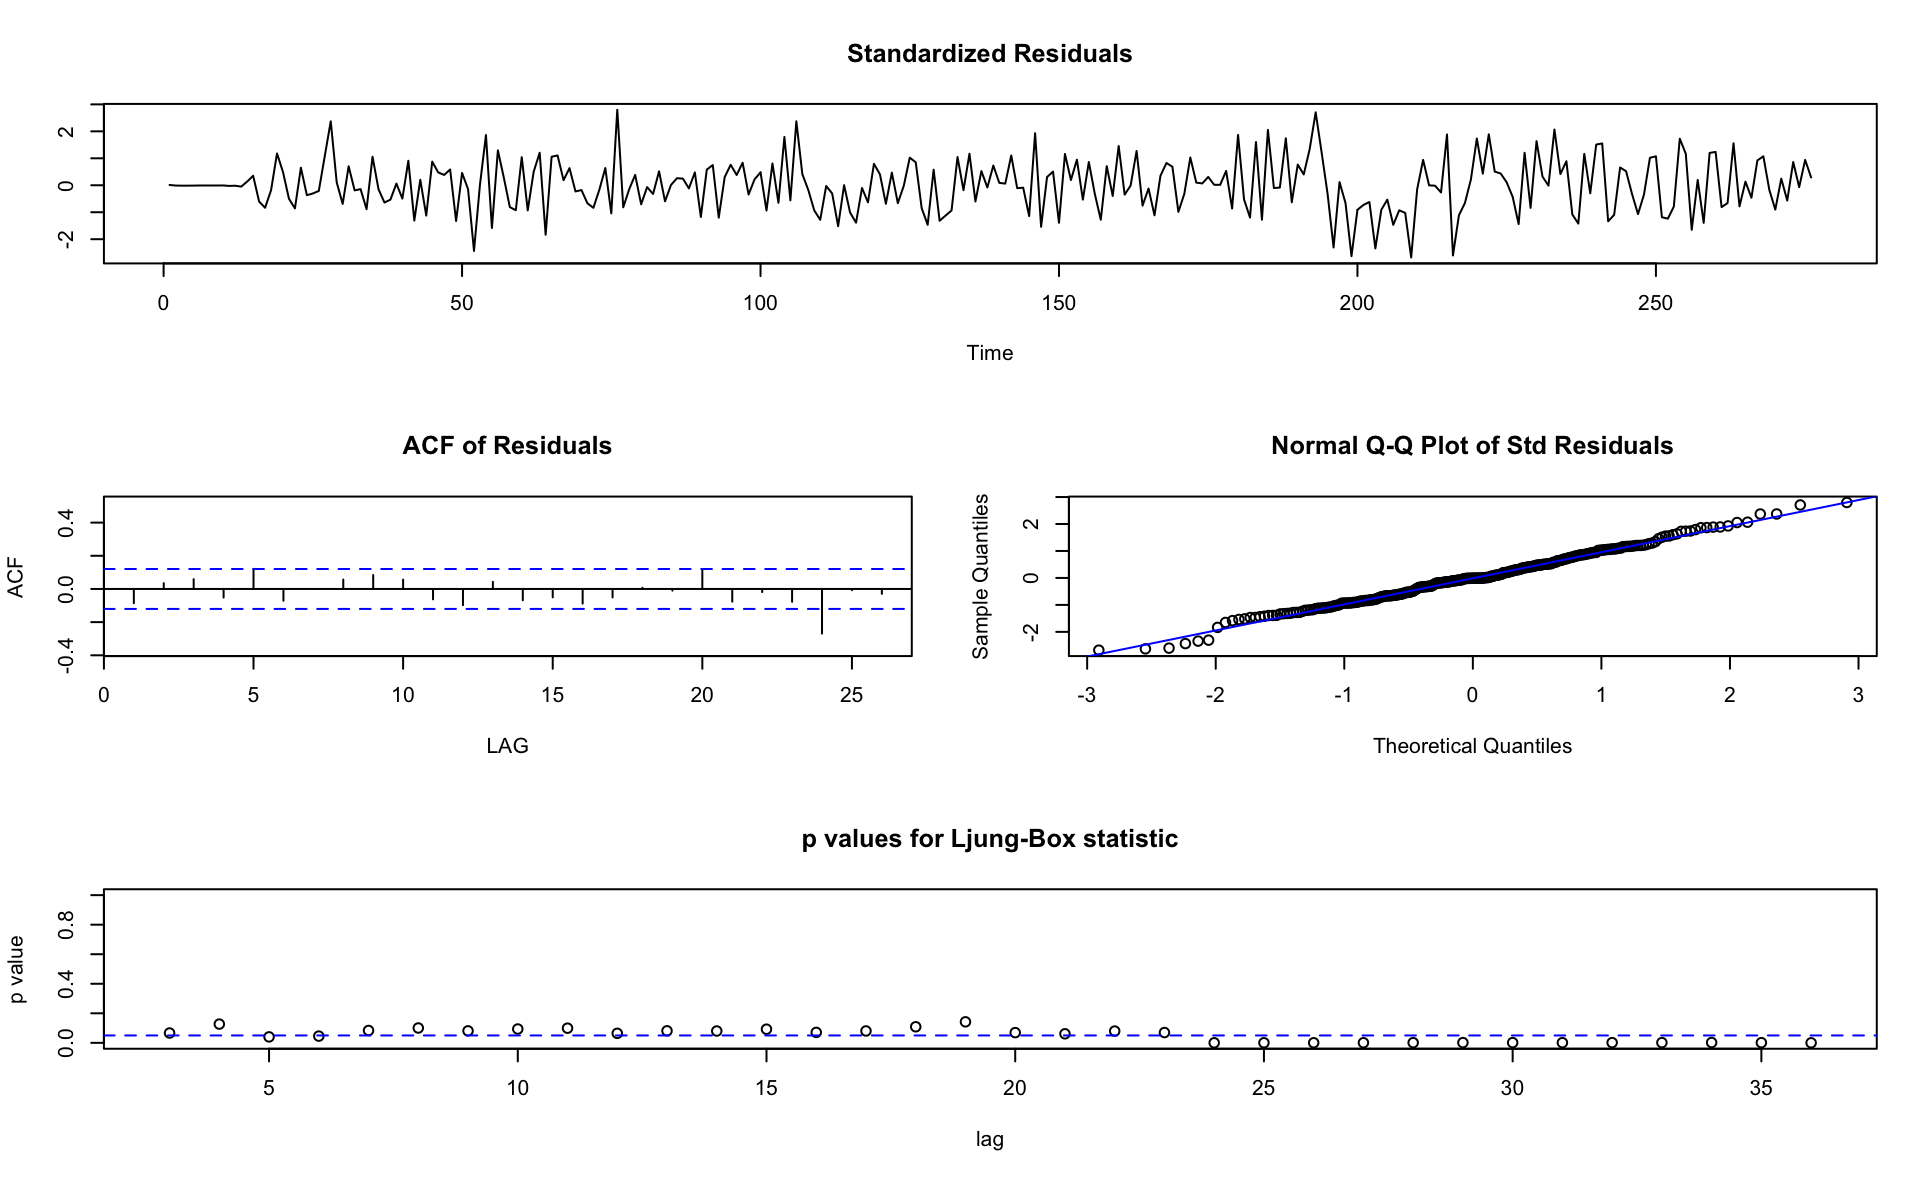
\includegraphics[width=\linewidth]{images/seasonalmodel1}
  \end{frame}

%-----------------------------------------------------------------------------------------

\begin{frame}{Model 2: SARIMA\((0,2,1) \times (3,1,0)_{12}\)}
  		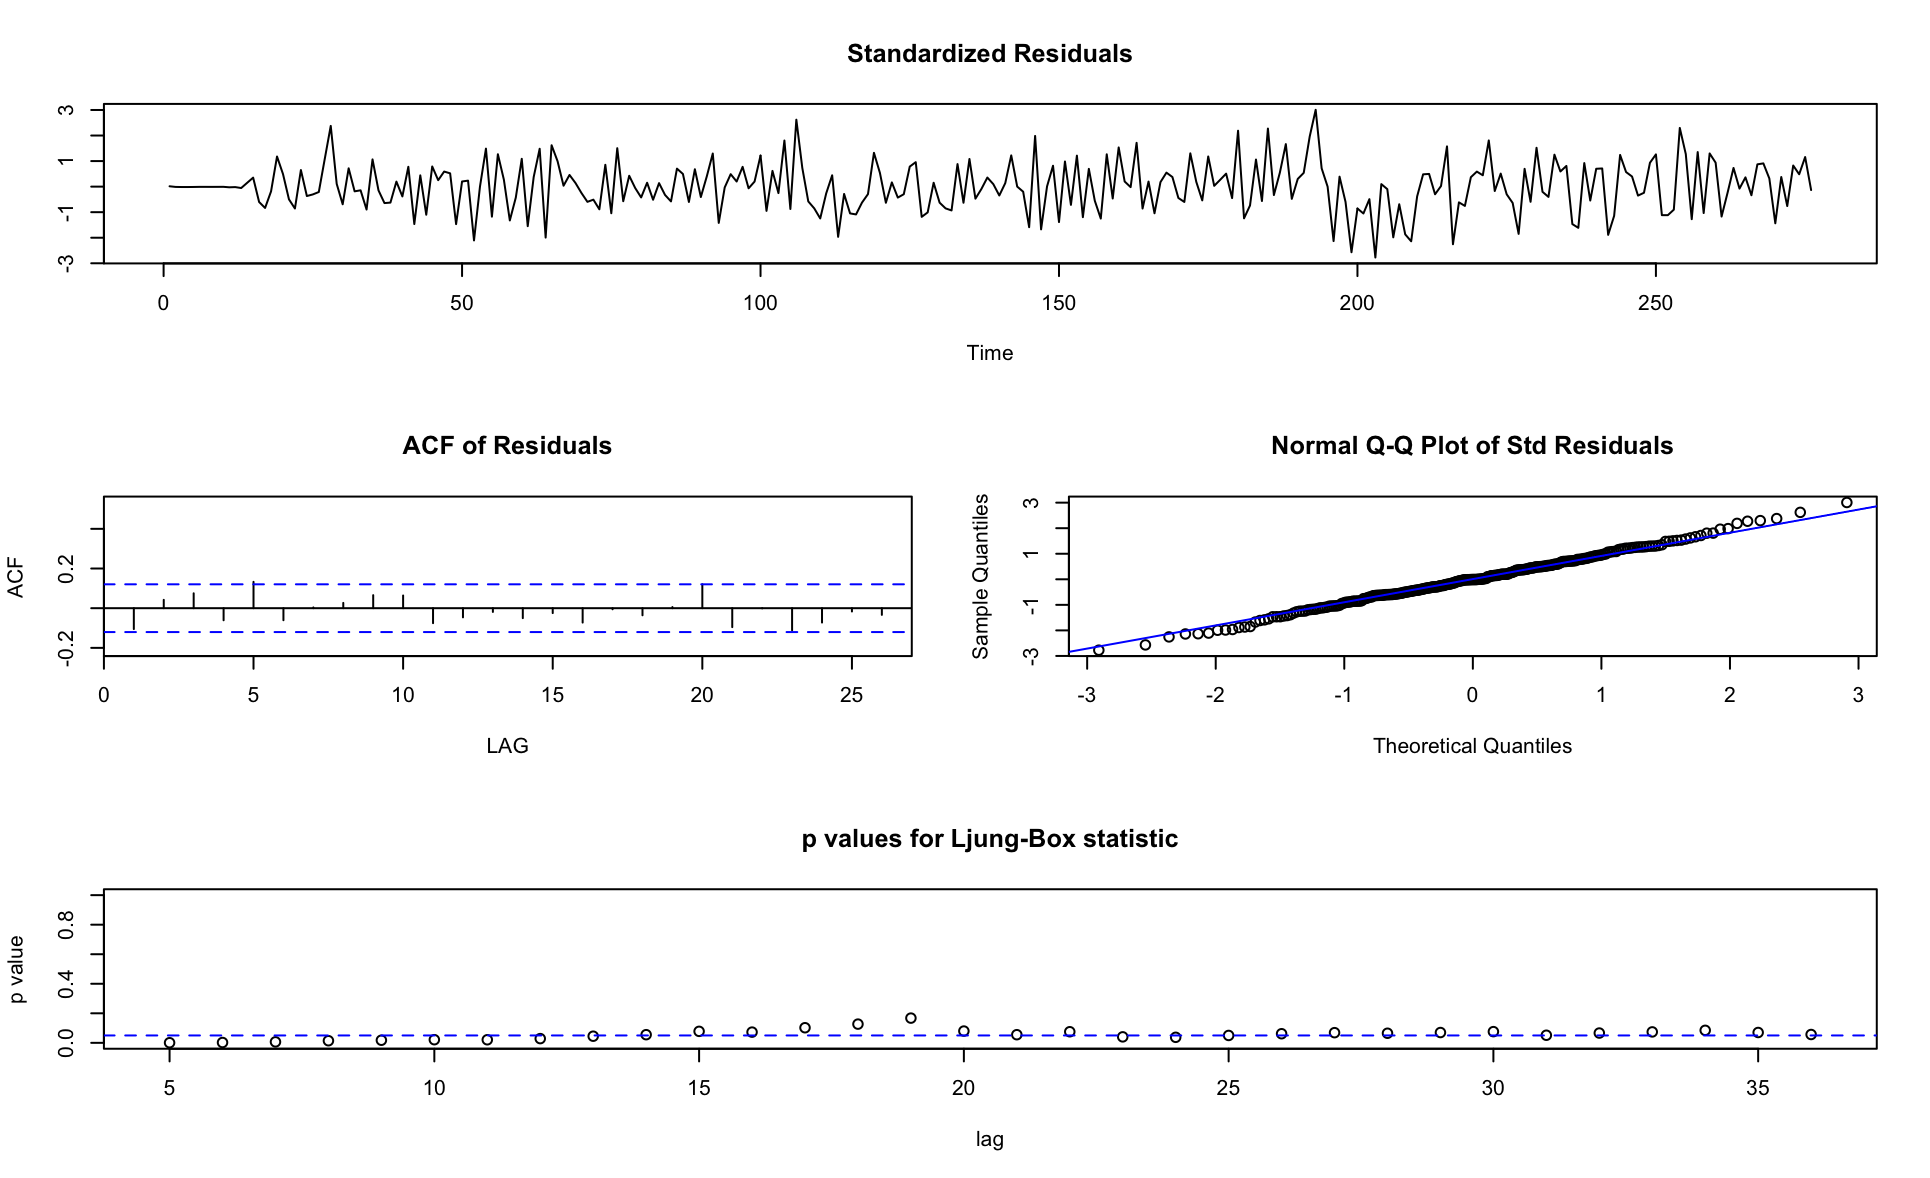
\includegraphics[width=\linewidth]{images/seasonalmodel2}
  \end{frame}  

%-----------------------------------------------------------------------------------------
  
  \begin{frame}{Model 3: SARIMA\((4, 2, 1) \times (3,1,0)_{12}\)}
  		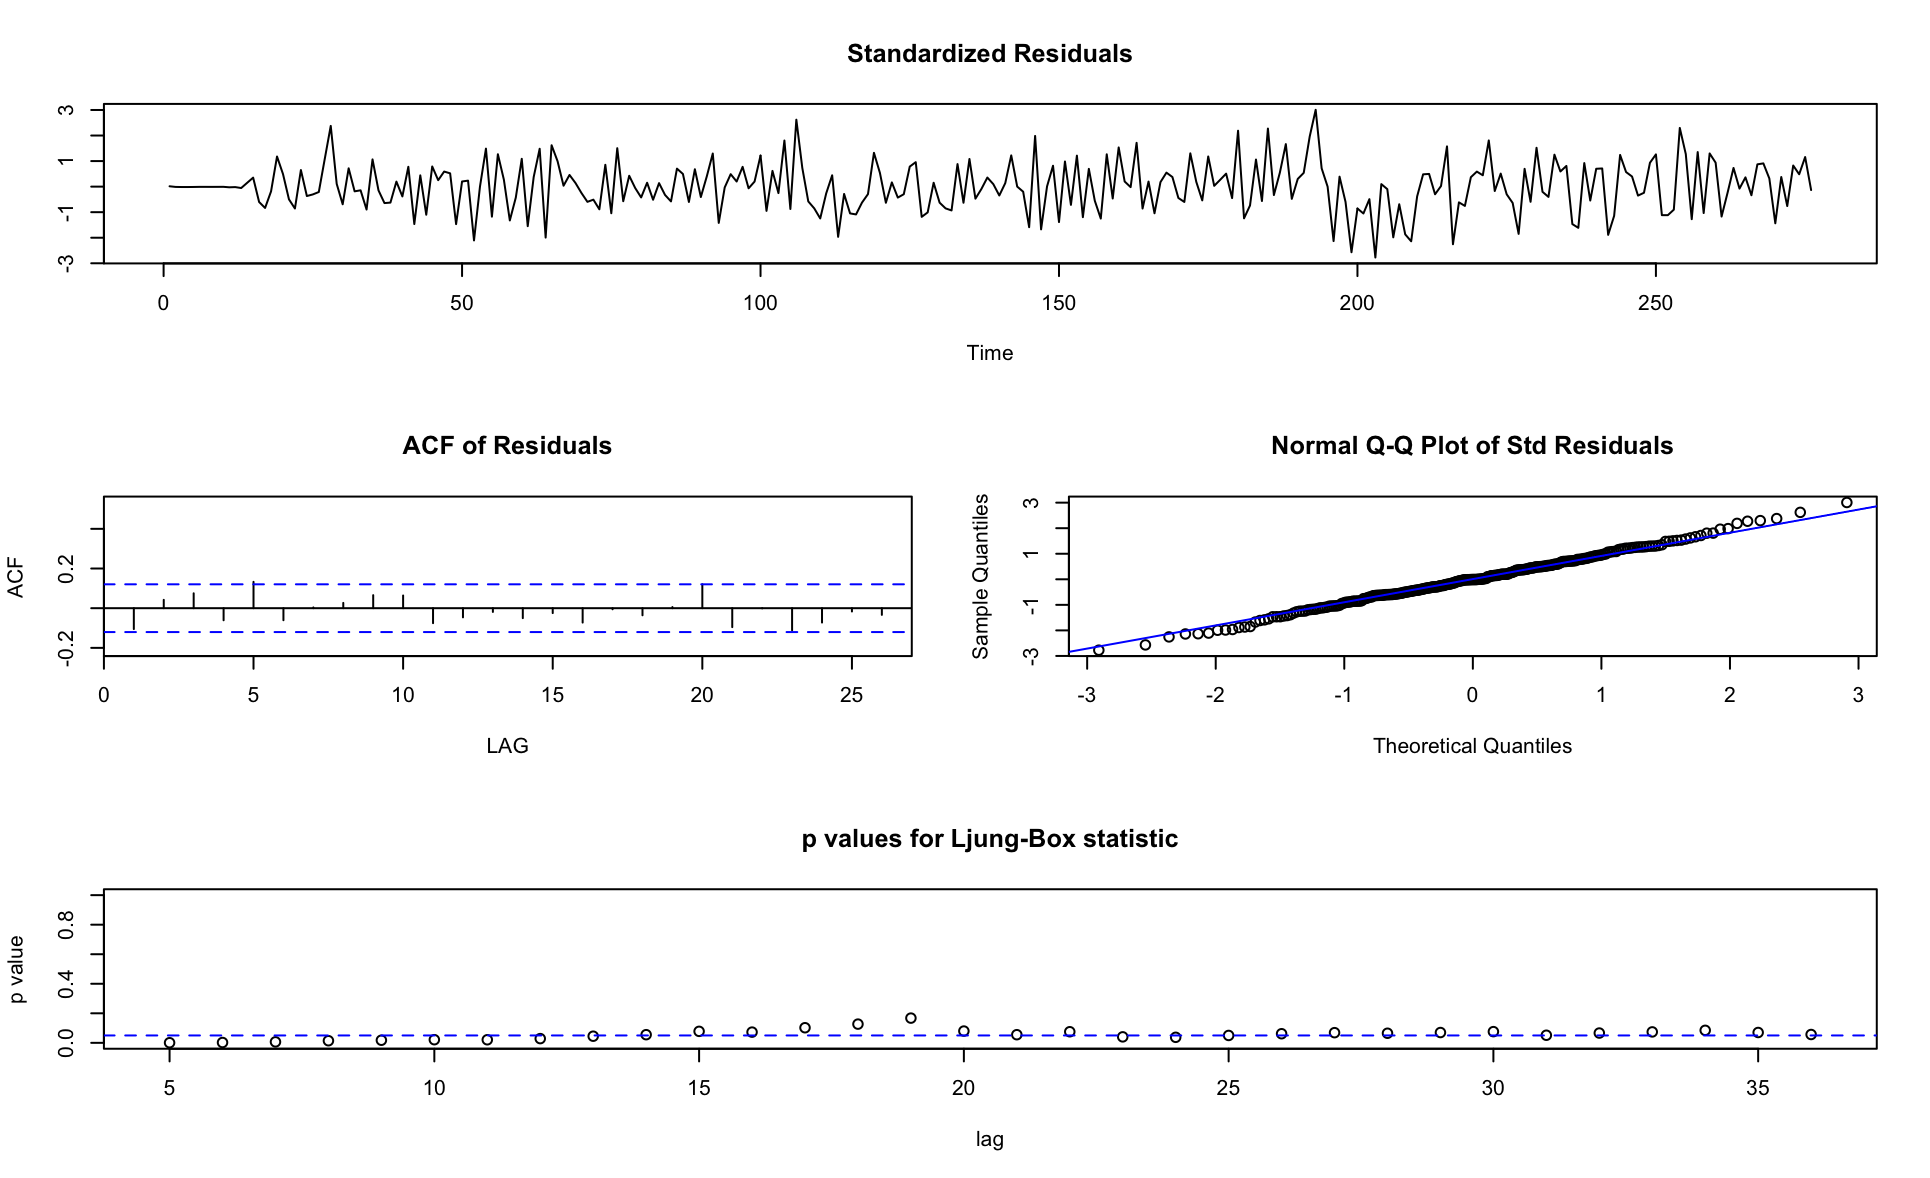
\includegraphics[width=\linewidth]{images/seasonalmodel3}
  \end{frame}  
%-----------------------------------------------------------------------------------------  

  \subsection{Seasonally Adjusted Models}
%-----------------------------------------------------------------------------------------  
  \begin{frame}{Model 4: SARIMA\((0,2,1) \times (1,0,0)_{12}\)}
  	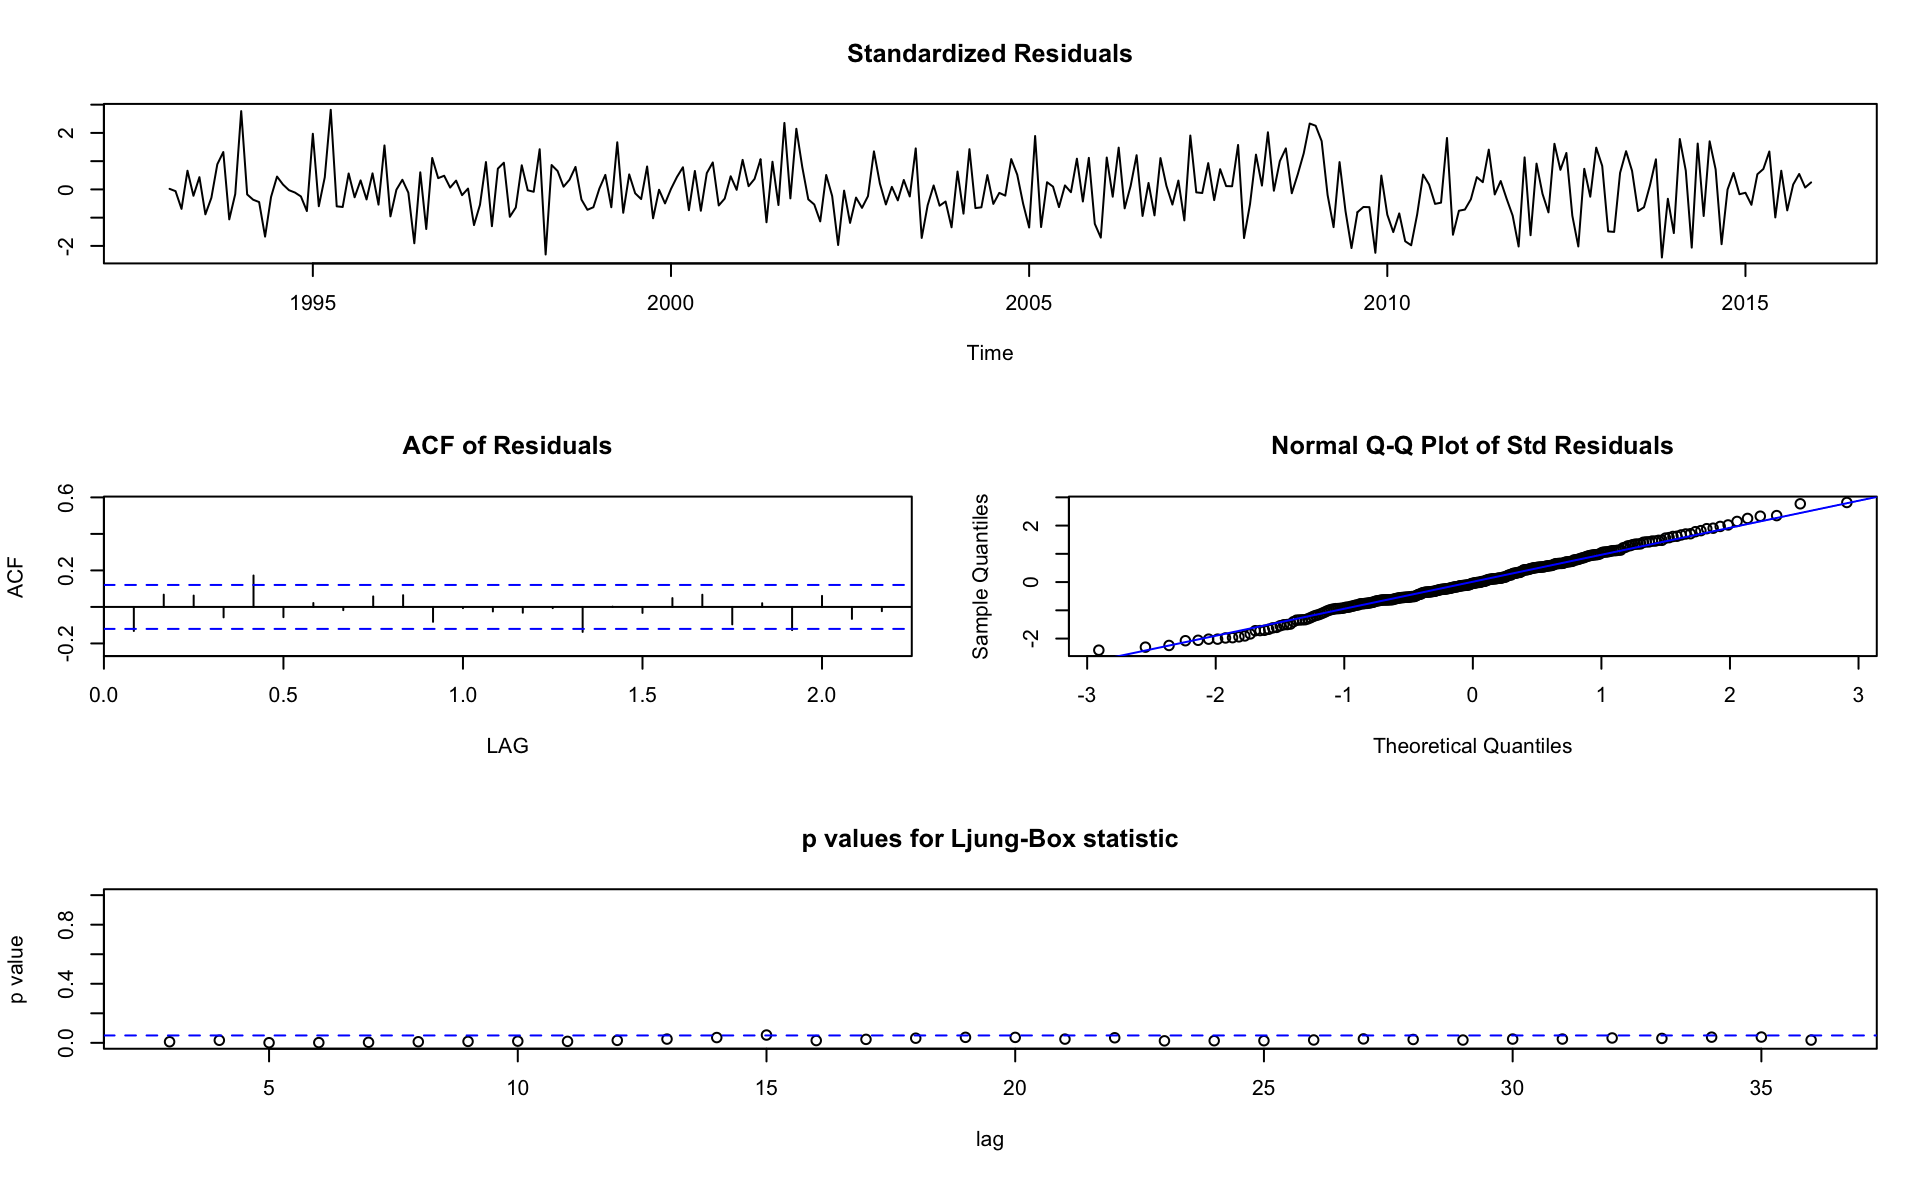
\includegraphics[width=\linewidth]{images/seasonallyadjustedmodel4}
  \end{frame}
  
%-----------------------------------------------------------------------------------------
  
  \begin{frame}{Model 5: ARIMA\((1,2,1)\)}
  		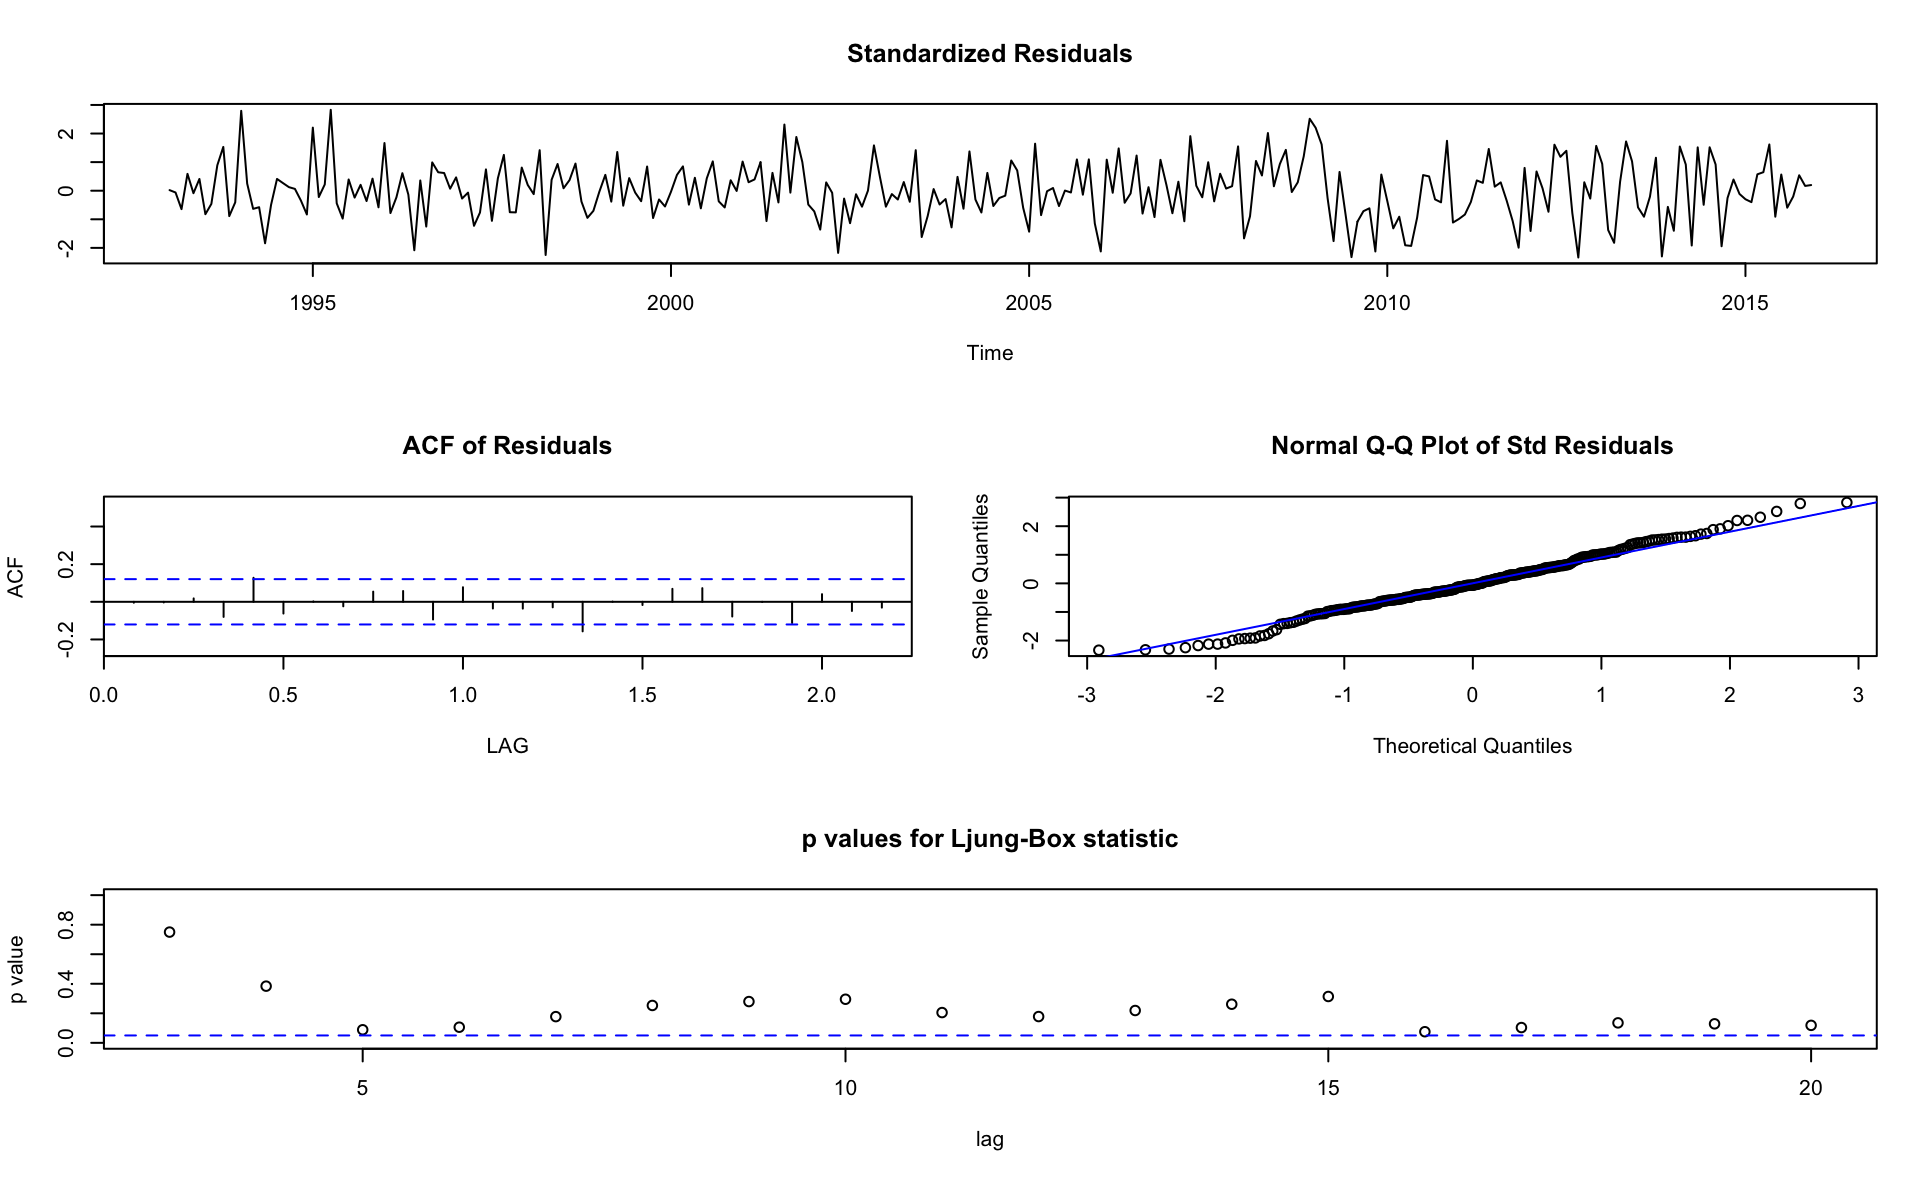
\includegraphics[width=\linewidth]{images/seasonallyadjustedmodel5}
  \end{frame}
  
  %-----------------------------------------------------------------------------------------
  
  \begin{frame}{Model 6: SARIMA\((0,2,1) \times (1,0,0)_{12}\) with Regressors}
  		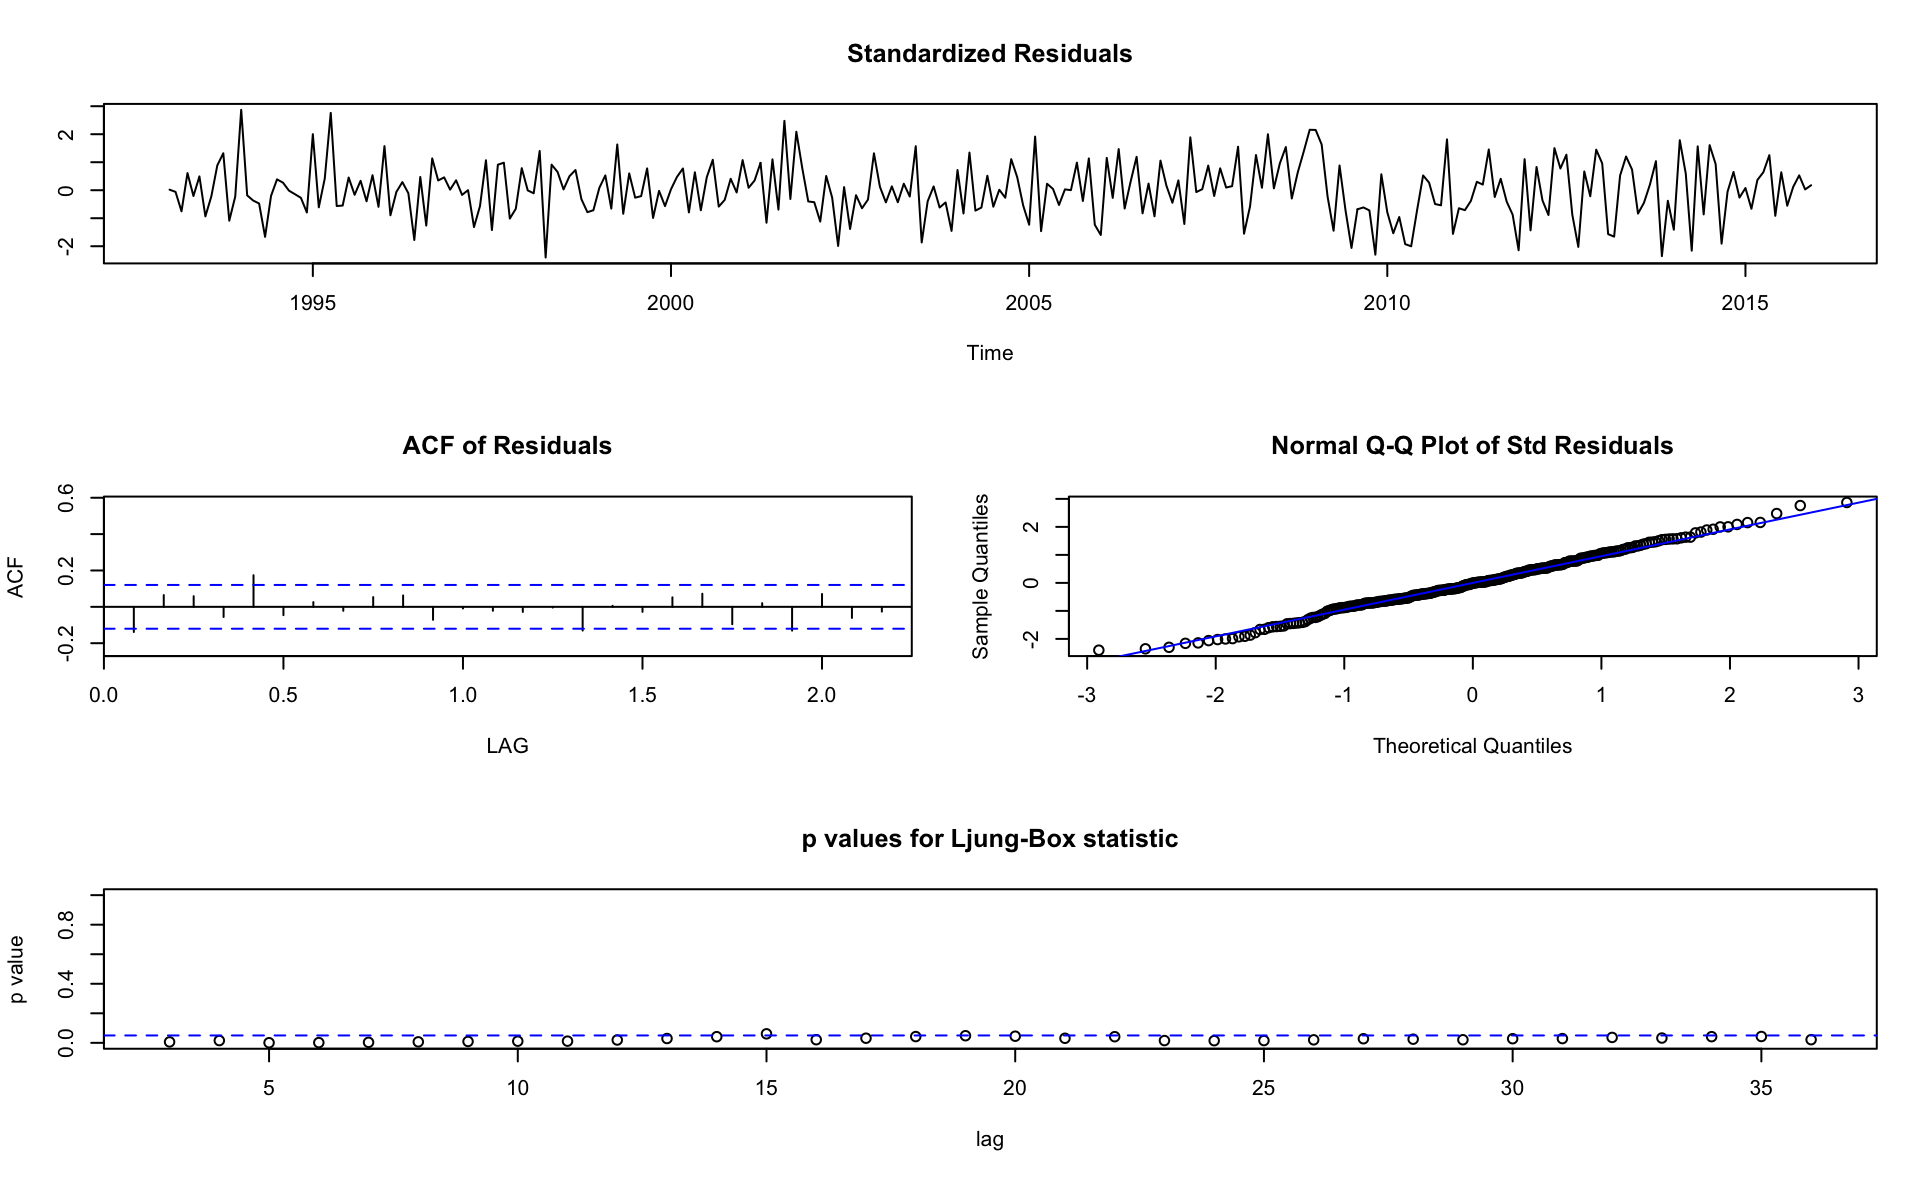
\includegraphics[width=\linewidth]{images/seasonallyadjustedmodel6}
  \end{frame}
  
  %-----------------------------------------------------------------------------------------
  
  \begin{frame}{Model 7: ARIMA\((1,2,1)\) with Regressors}
  		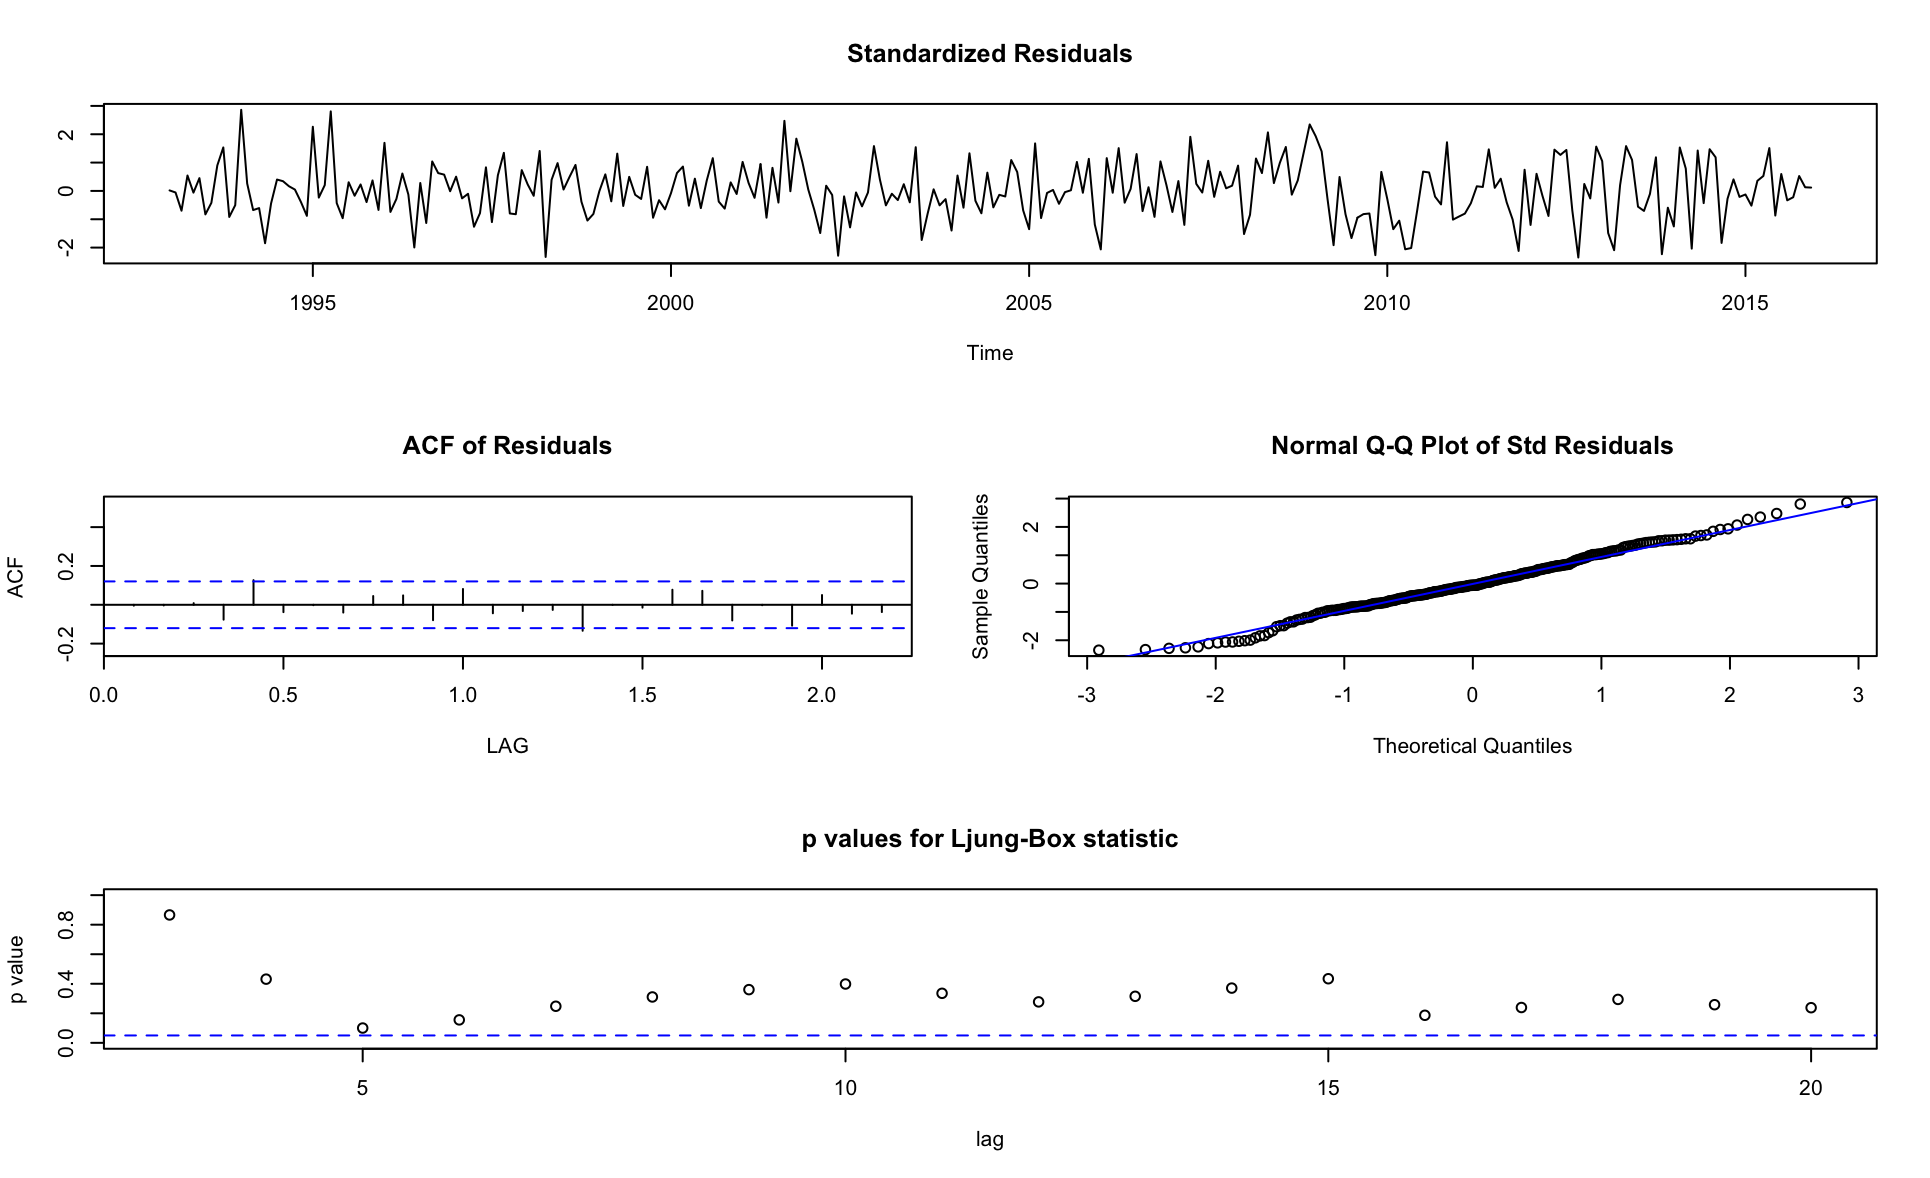
\includegraphics[width=\linewidth]{images/seasonallyadjustedmodel7}
  \end{frame}  
  
  
  From looking at AIC and BIC values, Models 2 and 3 perform quite similarly, which both show some slight evidence of outperforming Model1.\\
  
  Then we could compare the three models based on diagnostic plots. The standardized residuals of all models show some evidence of non-white-noise. ARMA models do not model variability. We will have a few lectures on this topic. There is not much we can do now on this issue.\\
  
  In the ACF of residuals of Model 1 shows a spike at lag 24. The other two models do not show such a spike.\\
  
  The normal plots from the three models are fairly similar.\\
  
  The Q-statistic or Ljung-Box statistic\\
  
  Models 1 and 2 have similar results. Model 1 seems to perform better at the first few lags, but Model 2 does better after lag 15. Model 3 clearly perform better than the two models on the Q-statistic. Since the Model 3 is based on a reasoning our professor does not like, we may not present this model. However it at least informs us that some models based on the thought that both the ACF and PACF cuts off at certain lags might model our data better. 
  %-----------------------------------------------------------------------------------------
  

\end{document}